% Diagrama de lo que espera hacer mi algorimto con una caja negra que es un sistema automl. Esperar que el sistema se actualize solo
% Escribir que es lo que espera mi algoritmo caja negra, y que es lo que retorna 
% Escribir como si todo fuera desde yo

\chapter{AutoML Multiobjetivo}\label{chapter:proposal}

Se propone como soluci\'on al  \textit{problema multiobjetivo en sistemas AutoML} (\ref{proposal:moo-automl-problem}) un algoritmo que utilize como caja negra un sistema de AutoML que pueda retornar un flujos y sus evaluaciones respecto a varias m\'etricas. Luego el programa selecciona los mejores utilizando un metodo de ordenaci\'on multiobjetivo y se los devuelve al sistema AutoML. Se espera que este, partiendo de los mejores flujos sea capaz de producir una nueva generaci\'on manteniendo estos rasgos. Se repite este paso hasta que se cumpla el criterio de parado, en donde se devuelven las mejores respuestas encontradas hasta el momento con respecto a todas las iteraciones.

\section{Descripci\'on General}
El sistema toma como entrada un sistema de Aprendizaje de M\'aquina Automatizado $\mathcal{A}$ tal que $\mathcal{A}(D, M, P) = TP$ donde $D = \{(x_1, y_1), (x_2, y_2), ..., (x_n, y_n)\}$ representa un conjunto de datos de entrada, $M = \{f_1, f_2, ..., f_m\}$ un conjunto de m\'etricas a evaluar y $P = \{p_1, p_2, ..., p_k\}$ una serie de modelos de Aprendizaje Autom\'atico por los cuales se gu\'ia $\mathcal{A}$ para producir una poblaci\'on $TP$. El objetivo del sistema es producir una serie de modelos de Aprendizaje Autom\'atico $P$ que sean una muestra representativa del frente de Pareto utilizando un algoritmo evolutivo multiobjetivo  $\mathcal{H}$ tal que $\mathcal{H}(TP) = P$. 

\begin{algorithm}[H]\caption{Flujo del Sistema}
    \KwIn{$\mathcal{A}$, D, M}
    \KwOut{P}
    
    $TP \gets \mathcal{A}(D, M, \emptyset)$ \tcp*{Se obtiene poblaci\'on inicial aleatoria}
    \While{no se cumplan condiciones de parada}{
        $P = \mathcal{H}(TP)$ \tcp*{Se extraen los m\'as aptos de una poblaci\'on} 
        $TP = \mathcal{A}(D, M, P)$ \tcp*{Se genera una nueva poblaci\'on}
    }
\end{algorithm}

\section{Sistema AutoML}
El sistema AutoML necesario para esta propuesta se utiliza como caja negra y debe ser capaz de producir una poblaci\'on inicial aleatoria, al igual que poblaciones que toman como base una serie de inidividuos para que los nuevos miembras conserven los rasgos de esto. Esto \'ultimo se logra utilizando algoritmos evolutivos que definen operadores de mutaci\'on, combinaci\'on y selecci\'on.

Nuestra propuesta est\'a basada en AutoGOAL (\cite{estevez2020solving}) un sistema de AutoML que modela el espacio de decisi\'on utilizando una Gram\'atica Probabil\'istica  Libre del Contexto (\textit{Probabilistic Context Free Grammar}, PCFG). 

Las PCFG se definen como una quinterna $PG = (NT, T, S, P, Prob)$ donde $NT$ y $T$ representan los conjuntos disjuntos no vac\'io de los s\'imbolos no terminales y terminales respectivamente. $S$ es un elemento de $NT$ llamado el axioma que representa el no-terminal inicial tal que expandiendo este se pueden llegar a todas las posibles formas de la gram\'atica. $P$ es el conjunto de reglas de producci\'on que rigen a la grma\'atica. $Prob$  es un conjunto de probabilidades asocaido con cada regla de la gram\'atica. 

Con el fin de aprovechar el espacio de decisi\'on ya definido se utiliza Evoluci\'on Gram\'atica Probabil\'istica (\textit{Probabilistic Grammatic Evolution}, PGE, \cite{megane2021probabilistic}), un algorimto de Estimaci\'on de Distribuci\'on (\textit{Estimation of Distribution ALgorithms, EDA}, \cite{larranaga2001estimation}) que remplaza los operadores cl\'asicos de mutaci\'on y cruce por un sampleado sobre las probabilidas de distribuci\'on de PCGG de acuerdo a las producciones utilizadas por el emjor individuo.

En PCFG, al inicio, las probabilidades est\'an igualmente distribuidas sobre todas las producciones por cada regla de la gram\'atica y se actualizan al aplicar PGE con el individuo m\'as apto donde se alterna entre aumentar ligeramente la probabilidad de las producciones que utilizadas por este y disminuir la probabilidades de los que no fueron utilizadas. Alternar entre estas dos v\'ias evita la utilizaci\'on del mismo individuo en iteraciones consecutivas balanceando la exploraci\'on global con explotaci\'on local.

\begin{algorithm}[H]\caption{Probabilistic Grammatical Evolution}
    \KwIn{fittest}
\end{algorithm}

Como se trata de un problema multiobjetivo y no existe el individuo m\'as apto, sino un conjunto de estos las probabilidas se adaptan secuencialmente teniendo en cuenta cada uno de estos individuos.
 % (\textit{Probabilistic Grammatic Evolution}).
% En PGE se propone un cambio de como se interpreta el genotipo, ya no es una lista de enteros, sino u
% Utiliza Algirmtos de Estimacion de Distribucion (\textit{Estimation of Distribution Algorithms, EDA}) una t\'ecninca probabi\'istica que remplaza los operadores de mutaci\'on y cruce por un sampleando sobre la probabiliad de distribuci\'on de las producciones obtenidas por mejor individuo, para luego generar una nueva poblaci\'on por cada cada generaci\'on. Las probabilidades comienzan todas inicializadas en igual proporci\'on  y se actualizan basado en la frecuencia de las reglas de produccion escogidas para obtener el individuo con el mayor rendimiento.
% Probablisitic Grammatical Evolution (PGE)  se apoya en una Gramatica Probabilistica Libre del Contexto (\textit{Probilistic Context-Free Grammatic Evolution} PCFGE) para realizar los mapeos de los fenotipos a los genotipos. PCFGE se establece como una tupla $PG = (NT, T, S, P, Prob)$ donde $Prob$  es un conjunto de probabilidades asocaido con cada regla de la gram\'atica. El genotipo en PGE es un vector de numeros fraccionarios, donde cada uno corresponer con la probabiliad de seleccion cierta regla de derivaci\'on.
% insetar ejemplo de PGE.
% En PGE las probabilidades se actualizan despues de cada generaci\'on  despues de evaluar la poblaci\'on generada, basasdo en cuantas veces cada regla de derivacion fue seleccionada por el el individuo de mejor rendimiento. Si la regla fue seleccionada su probablidad incrementa, en cambio si no, su probabilidad se reduce. Alternando entre estas dos variantes se ayuda a evitar usar el mismo individuo en iteraciones consecutivas, balanceando exploracion global con expotacion local.
% \subsubsection{GE}
% Con esta idea en mente nace Grammatical Evolution, que utiliza una gramatica para establecer restricciones sint\'acticas sobre las soluciones individuales. Introudce la distinci\'on entre el genotipo y el fenotipo. 
% Para obtener una soluci\'on se tienen el genotipo (usualmente una lista de enteros) que se mapea al fenotipo (una lista de prdoucciones) siguiendo las reglas de producci\'on en una Gram\'atica Libre del Contexto (\textit{Context-Free Grammar}, CFG). Donde una gramatica es una terna $G = (NT, T, S, P)$ donde $NT$ y $T$ representan los conjuntos disjuntos no vac\'io de los s\'imbolos no terminales y terminales respectivamente. $S$ es un elemento de $NT$ llamado el axioma que representa el no-terminal principal que expandiendo este se puede llegar a todas las posibles formas de la gramatica. $P$ es el conjunto de reglas de producci\'on que rigen a la grma\'atica. Las reglas en $P$ tienen la forma de $A ::= \alpha$, donde $A \in NT$ y  $\alpha \in (NT \cup F)^*$ 
% Insertar ejemplo de como funciona esta talla
% El rendimiento de GE ha sido criticado en la literatura por tener alta redundancia y poca localidad. Una representaci\'on tiene alta redundancia cuando varios genotipos corresponden al mismo fenotipo y localidad se refiere a como los cambios en el genotipo se refeljean en el fenotipo. Con el objetivo de mejora GE han exisitido varias propuestas. Una de esta es Evoluci\'on de Gram\'atica Probabilistica.
\section{MOEA basado en Frente de Pareto}

Cualquier algoritmo de este tipo es posible utilizarlo aqu\'i. La importancia radica en que los soluciones que se le den prioridad sean parte del frente de Pareto

% Explicar xq se quiere nsga2, xq esta probado, es un buen metodo de optimzacion estandar y demostrado
% Los nuevos metodos multiobjetivos se comparan con NSGAII.
\subsection{NSGA-II}

\begin{figure}[H]
    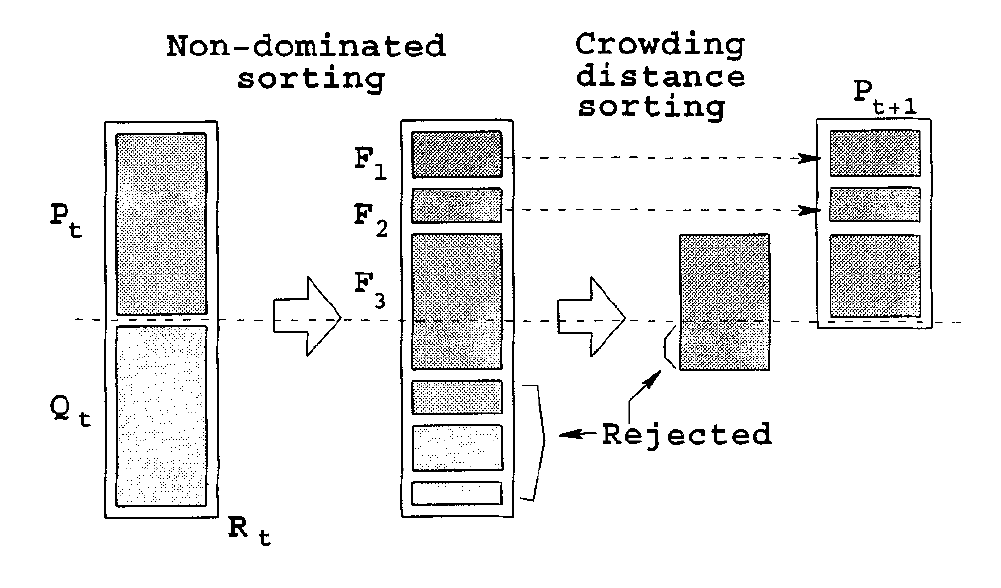
\includegraphics[width=\linewidth]{Pictures/nsga2.png}
    \label{nsga2}
\end{figure}

El funcinamiento general de NSGA-II es dado una poblacion ordenarlos, luego escoger los mejores $N$ individuos de dicha poblaci\'on y se genera una nueva poblacion con $2N$ individuos y se repiten los pasos.

La parte tocada de NSGA-II es en la manera en que ordena los elementos, que se divide en dos fases.

En la primera fase ordena las soluciones seg\'un las solucioens que las dominen, a traves de frentes de paretos de distinto rango. En primer lugar van las funciones que nadie domina, seria el frente de pareto de rango 0, las que domina al menos uno, el frente de pareto de rango 1, y as\'i sucesivamente.

Una vez se tenga esta ordenaci\'on se cogen los primero N soluciones para construir una nueva poblaci\'on a partir de esta utilizando un algoritmo gen\'etico. En el caso de que haya que picar por la mitad algun frente de rango K, es necesario utilizar otro metodo de ordenaci\'on. El objetivo final es obtener del frente de rango K la muestra mas representativa.

Para eso se propone Crowding distance:
Que calcula una estimaci\'on de la densidad de las soluciones vecinas a cierta soluci\'on. Se calcula el promedio de la distancia de estos dos puntos cercanos al punto por cada funci\'on objetivo. Esta distancia sirve como un estimado del perimetro del cuboide formado usando los vecinos m\'as cercanos como v\'ertices. 

El calculo de la distancia necesita ordenar la poblaci\'on de acuerdo a cada funcion objetivo en orden ascendiente. Las puntos de menor y mayor con respecto a una funci\'on objetivo son asignados $\infty$. Todas las soluciones intermedias son asignadas las distancias iguales a la diferencia absoulta normalizada de los valores de la funcion de dos puntos adyacentes. Este calculo se hace sobre todas las funciones objetivo. El crowding distance es calculado como la suma de cada distancia indivual correspondiendo a cada funci\'on objetivo.

\begin{algorithm*}\caption{Crowding Distance}
    l = |S|

    for i = 0 to l:

    \quad set S[i].distance = 0

    for each objective $m$

    \quad S = sort(S, m)

    \quad S[0].distance = S[l].distance = $\infty$

    \quad for i = 2 to (l - 1):

    \qquad 
    \begin{math}
        S[i].distance  = \frac{S[i].distance + (S[i + 1].m - I[i - 1].m)}{f^{max}_{m} - f^{min}_m}
    \end{math}
\end{algorithm*}


